\subsection{Sinus-förmige Projektion}
\label{sec:sinusodial}
Die Sinus-förmige Projektion ist eine flächentreue Projektion. Auch in dieser Projektion werden die Breitenkreise als Geraden dargestellt. Das besondere an der Sinus-förmigen Projektion ist das die Länge der Breitenkreise relational zu $\cos\varphi$ ist, dies führt zu einer starken Verzerrung außerhalb der Mitte.\\
Vorteil der Sinus-förmigen Projektion:\\
\begin{itemize}
\item Die Projektion ist einfach zu berechnen.
\end{itemize}
Nachteil der Sinus-förmigen Projektion:\\
\begin{itemize}
\item Die Projektion ist nicht sehr anschaulich.
\end{itemize}
Formel:\\
\begin{eqnarray*}
\mathcal {X} & = &\cal{R}\cdot(\lambda - \lambda _0)\cdot \cos \varphi \\
\mathcal{Y} & = &\cal{R} \cdot \varphi
\end{eqnarray*}

\begin{figure}[hbtp]
\centering
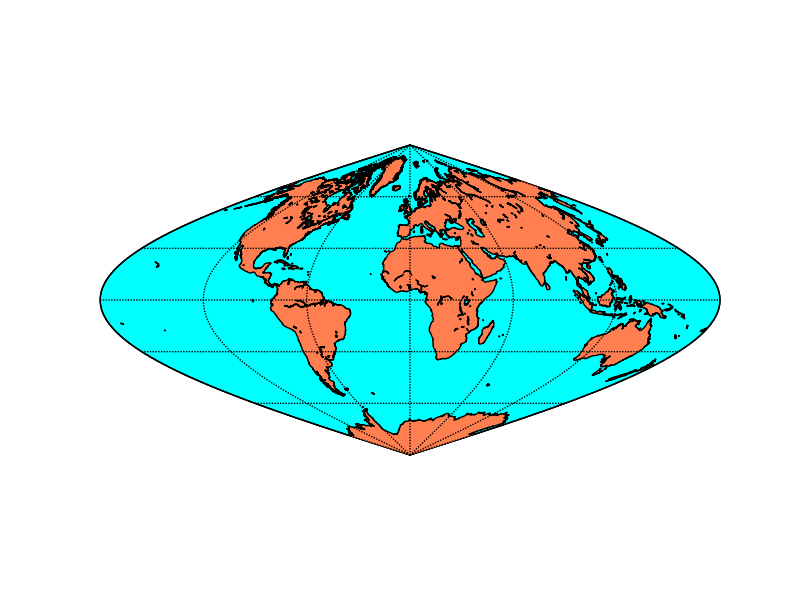
\includegraphics[scale=0.5,origin=c]{/Users/student/seminar/Kartendarstellungen/seminar/sinu} 
\caption{Sinus-förmige Projektion}
\end{figure}
\newpage 